\chapter{Estructura y funcionamiento del sistema completo} \chapterlabel{Estructura-sist} \label{cap:estructura sist}

\section{Introducción}
El propósito de este proyecto final es diseñar un prototipo a partir del cual la empresa pueda continuar con su desarrollo y obtener un producto. La versión comercial pensada a futuro en conjunto con la empresa puede observarse en el esquema de la figura \ref{fig:img_croquis-est}.

El objetivo de este capítulo es describir la estructura y funcionamiento del sistema completo a partir del cual se desarrollará el prototipo final.

\begin{itemize}
	\item \textcolor{mGreen}{Este no es el definitivo, ya que tiene los colores invertidos y líneas del AutoCAD.}
	\end{itemize}

\begin{figure}[H]
	\centering
	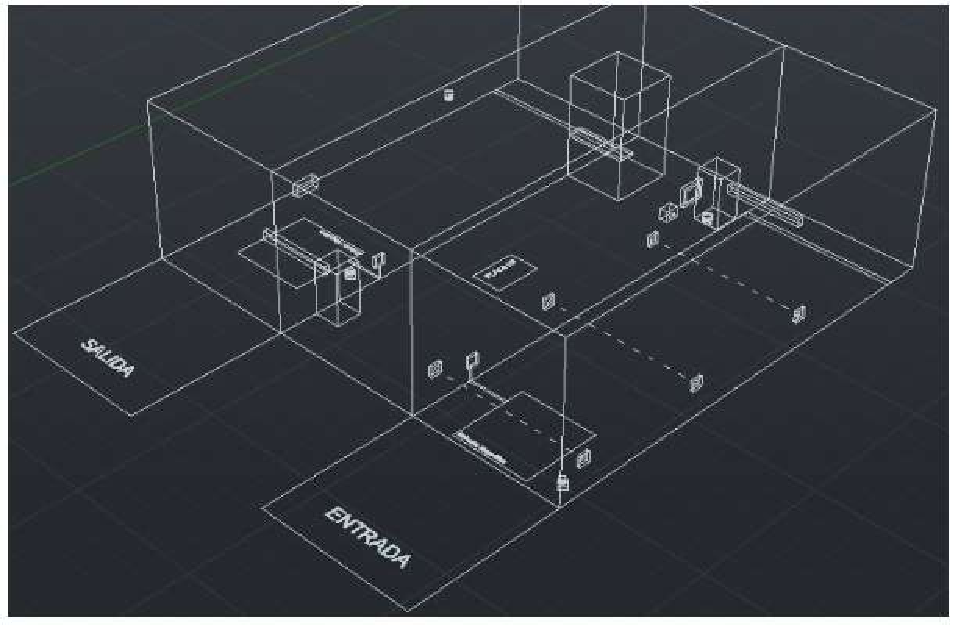
\includegraphics[width=\textwidth]{croquis.pdf}
	\caption{Producto pensado a futuro.}
	\label{fig:img_croquis-est}
\end{figure}

El sistema final fue planteado para un estacionamiento como el de la figura \ref{fig:img_croquis-est}, con vías de ingreso y egreso independientes. Sin embargo, el mismo es fácilmente adaptable a establecimientos que posean características diferentes. 

Basándonos en este modelo, el sistema posee tanto en el ingreso como en el egreso, una barrera vehicular, un detector magnético de presencia y dos cámaras IP.  Se utilizan dos cámaras debido a que las motocicletas no poseen patente delantera, mientras que los demás vehículos sí. Entonces, una apunta a la patente trasera y la otra a la delantera.

Además, en el ingreso se encuentra un mecanismo de detección de tipo (o tamaño) de vehículo implementado con tres barreras infrarrojas. Las mismas funcionan en conjunto con el detector magnético. En la vía de entrada se cuenta también con una pantalla que indica a los clientes el lote asignado y la información que el encargado del establecimiento desee mostrar, y una impresora de tickets internos al estacionamiento con código de barra.

Por último, dentro de la cabina del operador del sistema, se tiene la Unidad Central de Control (UCC), encargada de interactuar con todos los componentes del sistema y procesar los datos obtenidos por los mismos. Entre las tareas que desarrolla se encuentran obtener el número de la patente del vehículo que ingresa o egresa del estacionamiento y de gestionar la base de datos. Además, en la cabina también se cuenta con una impresora de tickets fiscales y un lector de código de barra.
 
Uno de los componentes fundamentales del sistema es la Placa I/O \hl{CAMBIAR NOMBRE DE LA PLACA} que concentra todos los periféricos de la zona de ingreso/egreso, menos las cámaras, y que se comunica con la UCC  mediante WI-FI.

\section{Funcionamiento}

En la figura \ref{fig:img_img-china} puede observarse el esquema de funcionamiento del sistema a un nivel general. El mismo se explica más detalladamente a lo largo de las dos siguientes secciones.

\begin{figure}[H]
	\centering
	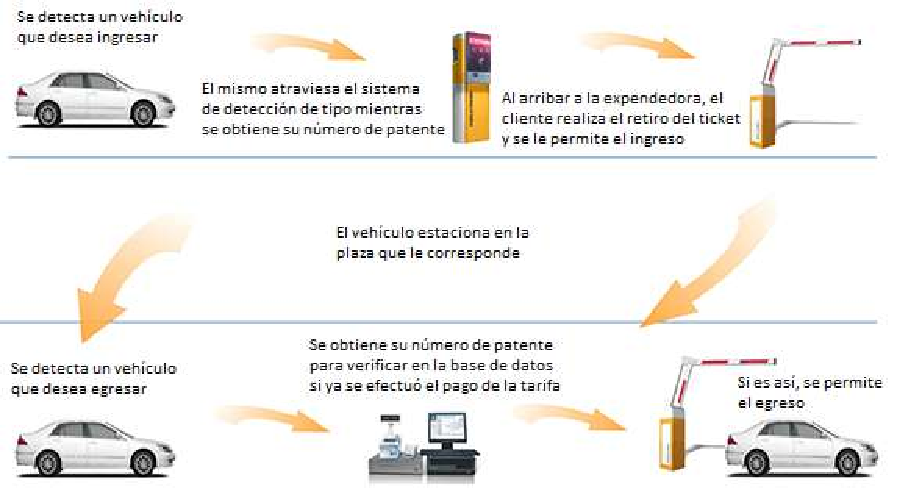
\includegraphics[scale=1]{img-china.pdf}
	\caption{Esquema general de funcionamiento del sistema.}
	\label{fig:img_img-china}
\end{figure}

A continuación, se describen los módulos de ingreso y egreso del sistema.

\subsection{Ingreso}

Como se observa en la figura \ref{fig:img_ingreso}, el proceso comienza con la detección de un vehículo que desea ingresar al estacionamiento. La misma se realiza mediante un detector magnético ubicado en el suelo, bajo el pavimento. Este posee una bobina (el lazo) cuya inductancia varía cuando un gran elemento metálico se acerca a ella. Esa variación hace que se modifique la frecuencia de oscilación del oscilador que posee el equipo. Esto produce la activación de un contacto seco que se utiliza para indicarle al sistema que un vehículo intenta ingresar al establecimiento.

\begin{figure}[H]
	\centering
	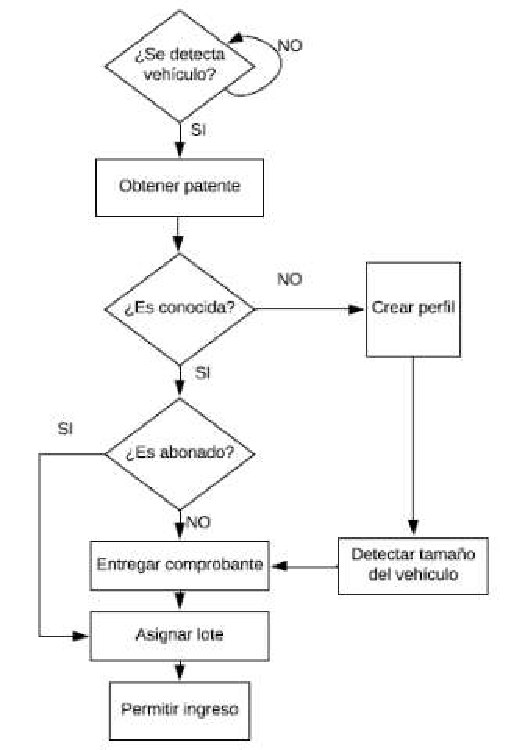
\includegraphics[scale=1]{func-ingreso.pdf}
	\caption{Funcionamiento del sistema en el ingreso.}
	\label{fig:img_ingreso}
\end{figure}

A continuación, se realiza la obtención de la patente mediante un juego de dos cámaras IP que se encuentran filmando continuamente. La misma es buscada en la base de datos y, en caso de no ser encontrada, se crea un perfil para el vehículo. Además, se determina el tamaño del mismo y se lo añade al perfil, con el objetivo de determinar la tarifa a cobrar (automóvil, camioneta o motocicleta). 

Luego, se procede a asignarle al conductor, mediante una pantalla, el lote en el que debe estacionarse, la hora de ingreso, la patente y la tarifa. Junto a la pantalla se encuentra una expendedora de tickets internos al estacionamiento, que poseen un código de barra y la misma información mostrada anteriormente. Los mismos se pueden retirar sin bajarse del vehículo. 

En caso de que el usuario sea abonado, no se le entrega el ticket debido a que el sistema reconoce la condición de abonado al detectar la patente.

Luego de que el usuario retire el ticket, se levanta la barrera y se permite el acceso. 


\subsection{Egreso}

Al igual que el de entrada, el sistema de egreso comienza con la detección de un vehículo que desee retirarse del establecimiento. El mismo puede observarse en la figura \ref{fig:img_egreso}. Una vez que esto sucede, se procede a obtener la patente del vehículo, con el fin de determinar si la tarifa ya fue pagada.

\begin{figure}[H]
	\centering
	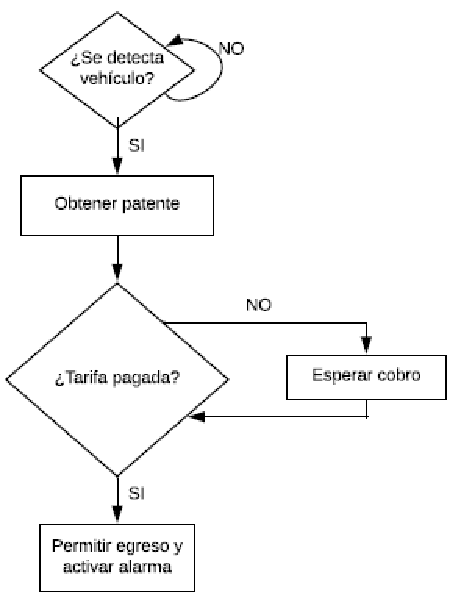
\includegraphics[scale=1]{func-egreso.pdf}
	\caption{Funcionamiento del sistema en el egreso.}
	\label{fig:img_egreso}
\end{figure}

Mediante un lector de códigos de barra ubicado en la cabina del operario se reconoce el horario de ingreso a partir del ticket de entrada, se determina el tiempo de uso del servicio y, por lo tanto, el monto a cobrarle al cliente.

Después de realizar el pago, a cada cliente se le entrega un comprobante con validez legal y se le permite el egreso. Sí el sistema comprueba que el cliente aún no realizó el pago, no le permite la salida hasta que esto suceda.

En el caso de los abonados, al detectar la patente el sistema verifica que la tarifa haya sido pagada. De ser así, se permite el egreso.

Se implementa una alarma luminosa y sonora para indicar el egreso de los vehículos.


\section{Relevamiento de estacionamientos}
%\hl{Esto lo pondr\'ia en otro cap\'itulo}

El diseño del estacionamiento de prueba presentado en la figura \ref{fig:img_croquis-est} fue construido en base a los resultados del relevamiento de una muestra (que se consideró representativa) de estacionamientos ubicados en la ciudad de Mar del Plata. Este relevamiento permitió definir qué aspectos considerar en el prototipo para cubrir las necesidades de automatización real y de interés para la empresa solicitante del sistema.

Los establecimientos inspeccionados se encuentran en diferentes zonas de la ciudad, poseen distintas características edilicias, son de diferentes capacidades y disponen de distintos sistemas de atención al cliente y de control de acceso. Además, mientras que en algunos estacionamientos se ingresó y se conversó con el personal a cargo, en otros se realizaron inspecciones visuales desde el exterior de los mismos. 

Entre las características que se tuvieron en cuenta al hacer el relevamiento se encuentran:
\begin{itemize}
	\item El equipamiento con el que contaban: barreras, cámaras e iluminación
	\item Mecanismo de detección de llegada de los vehículos
	\item Características edilicias: techo y condición del piso (podría afectar la toma de fotos)
	\item Si la vía de entrada-salida era una sola o si existían dos independientes
	\item Disposición del espacio en la zona de ingreso-egreso
\end{itemize}

\subsection{Equipamiento disponible}
A continuación, se presentan tres tablas junto con tres graficos de torta que muestran los resultados del relevamiento respecto al equipamiento disponible en los dieciséis establecimientos inspeccionados. En la tabla \ref{tabla:est_con_barr} (fig. \ref{fig:img_torta1-2-3} a) se observa la proporción de estacionamientos que poseen y no poseen barreras, en la tabla \ref{tabla:est_ilum} (fig. \ref{fig:img_torta1-2-3} b) se muestra cómo es la iluminación de los mismos y, finalmente, en la tabla \ref{tabla:est_cam} (fig. \ref{fig:img_torta1-2-3} c) se presenta la proporción de establecimientos que cuentan y de los que no cuentan con cámaras de video.

\begin{table}[htbp]
	\begin{center}
		\begin{tabular}{|c|c|c|}
			\hline
			Barrera & Sí & No\\
			\hline \hline
			Proporción de estacionamientos & 12.5\% & 87.5\% \\ \hline
		\end{tabular}
		\caption{Proporción de estacionamientos que poseen y no poseen barrera.}
		\label{tabla:est_con_barr}
	\end{center}
	\quad
	\begin{center}
		\begin{tabular}{|c|c|c|c|}
			\hline
			Iluminación & Artificial & Artificial + Natural & Natural\\
			\hline \hline
			Proporción de estacionamientos & 87.5\% & 6.25\% & 6.25\%\\ \hline
		\end{tabular}
		\caption{Característica de la iluminación de los estacionamientos relevados.}
		\label{tabla:est_ilum}
	\end{center}
	\quad
	\begin{center}
		\begin{tabular}{|c|c|c|}
			\hline
			Cámaras & Sí & No\\
			\hline \hline
			Proporción de estacionamientos & 43.75\% & 56.25\% \\ \hline
		\end{tabular}
		\caption{Proporción de estacionamientos que poseen y no poseen cámaras de video.}
		\label{tabla:est_cam}
	\end{center}
\end{table}


\begin{figure}[htb]
	\centering
	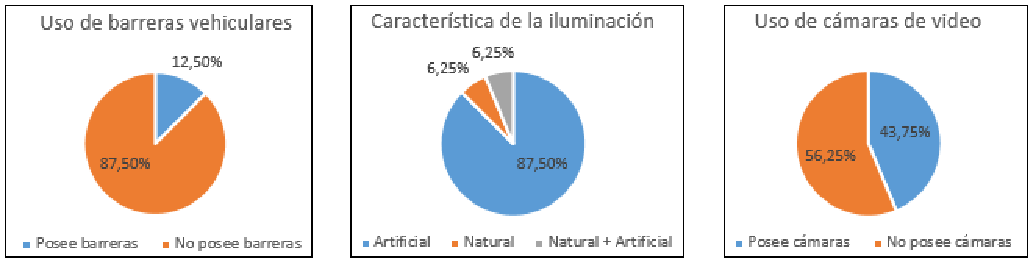
\includegraphics[width=\textwidth]{torta1-2-3a.pdf}
	\caption{Proporciones de: (a) los establecimientos que poseen y no poseen barreras, (b) de las características de la iluminación en los mismos y (c) de estacionamientos que utilizan o no cámaras de video.}
	\label{fig:img_torta1-2-3}
\end{figure}



Los estacionamientos de la ciudad que actualmente poseen cámaras de video no las utilizan para el mismo propósito que se les da en este proyecto. En la mayoría de ellos son usadas por cuestiones de seguridad, para observar la llegada de los vehículos o para ambas simultáneamente (varias cámaras con diferentes propósitos).

\subsection{Mecanismo de detección de los vehículos}
En esta sección, se presenta la forma en que se realiza la detección del vehículo en los accesos de los estacionamientos relevados. Esto se muestra en la tabla \ref{tabla:est_dec_det}, que se encuentra acompañada por el gráfico de la figura \ref{fig:img_torta4a}.

\begin{table}[h]
	\begin{center}
		\resizebox{14cm}{!} {
			\begin{tabular}{|c|c|c|c|c|} 
				\hline
				Mec. Detección & \parbox{3cm}{\centering Visualmente \\ (operador)} & \parbox{4cm}{\centering Visualmente \\
					(operador + cámaras)}
				& \parbox{3cm}{\centering Detector \\ magnético} & Botón\\
				\hline \hline
				\parbox{3cm}{\centering Proporción de \\ estacionamientos} & 62.5\% & 25\% & 6.25\% & 6.25\%\\ \hline
			\end{tabular}
		}
		\caption{Proporción de los mecanismos de detección utilizados en los estacionamientos.}
		\label{tabla:est_dec_det}
	\end{center}
\end{table}

\begin{figure}[htb]
	\centering
	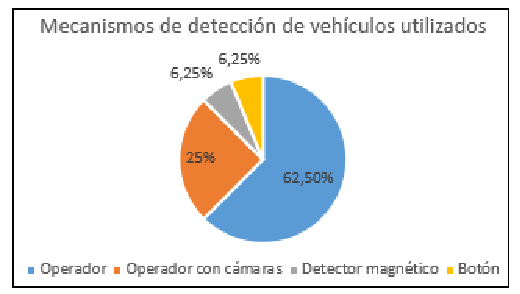
\includegraphics[scale=1]{torta4a.pdf}
	\caption{Proporciones de los tipos de mecanismos de detección de vehículos utilizados.}
	\label{fig:img_torta4a}
\end{figure}

La primera categoría hace referencia al caso en el que la detección implica que un operador se encuentra vigilando en forma visual el ingreso al establecimiento constantemente. Debido a esto, en la mayoría de los estacionamientos la cabina del operador es vidriada y se encuentra en una zona cercana a las vías de entrada-salida.

La segunda categoría se refiere a que la persona encargada de la operación del establecimiento cuenta con un sistema de cámaras apuntando hacia las vías de ingreso-egreso. Esto le permite a la misma visualizar cuando un vehículo entra o sale del establecimiento en un monitor dentro de la cabina. En este caso, esta última puede encontrarse alejada de los accesos al estacionamiento. 

La última categoría considera el uso de detectores magnéticos en los ingresos. Estos detectan la circulación de un vehículo debido a las variaciones magnéticas que el contenido ferroso de los automóviles les provoca. 

\subsection{Techo y piso}
A continuación, se muestra la proporción de estacionamientos techados y al aire libre, junto con información acerca del piso utilizado en los mismos. Esto puede observarse en las tablas \ref{tabla:est_techo} y \ref{tabla:est_piso}, que se encuentran acompañadas por los gráficos de la figura \ref{fig:img_torta5-6a}.

Debido a que se plantea un estacionamiento de prueba que sea adaptable a la mayor cantidad de escenarios posible, es importante conocer estas proporciones. Además, es necesario determinar las características del piso que generalmente se utiliza en este tipo de establecimientos. Esto se debe a que hay que asegurar que el sistema no tenga problemas con el mismo al fotografiar las chapas patentes.

\begin{table}[htbp]
	\begin{center}
		\begin{tabular}{|c|c|c|}
			\hline
			Estacionamiento techado & Sí & No\\
			\hline \hline
			Proporción de estacionamientos & 87.5\% & 12.5\% \\ \hline
		\end{tabular}
		\caption{Proporción de estacionamientos techados y al aire libre dentro de la muestra.}
		\label{tabla:est_techo}
	\end{center}
	\quad
	\begin{center}
		\begin{tabular}{|c|c|c|}
			\hline
			Tipo de piso & Cemento liso & Otro\\
			\hline \hline
			Proporción de estacionamientos & 87.5\% & 12.5\% \\ \hline
		\end{tabular}
		\caption{Proporción de estacionamientos según el tipo de piso.}
		\label{tabla:est_piso}
	\end{center}
\end{table}

\begin{figure}[htb]
	\centering
	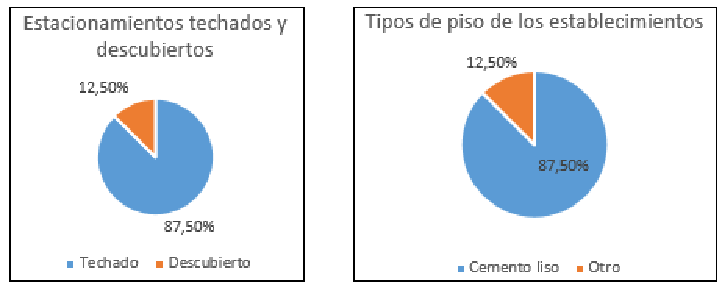
\includegraphics[scale=1]{torta5-6a.pdf}
	\caption{Proporciones de: (a) los establecimientos techados y descubiertos y (b) de los tipos de piso utilizados.}
	\label{fig:img_torta5-6a}
\end{figure}

%\begin{table}[htbp]
%	\begin{center}
%		\begin{tabular}{|c|c|c|}
%			\hline
%			Tipo de piso & Cemento liso & Otro\\
%			\hline \hline
%			Proporción de estacionamientos & 87.5\% & 12.5\% \\ \hline
%		\end{tabular}
%		\caption{Proporción de estacionamientos según el tipo de piso.}
%		\label{tabla:est_piso}
%	\end{center}
%\end{table}

Cabe destacar que en los dos establecimientos en el que el piso no es cemento liso se cuenta con un piso de tierra y uno compuesto por baldosas cerámicas blancas. Este último podría afectar a las cámaras debido a que puede reflejar la luz.

\subsection{Característica de las vías de entrada-salida}
En esta sección, se pretende determinar si existe una única vía utilizada para ambos propósitos o si existen dos rutas independientes. Es necesario conocer esta información debido a que el equipamiento del sistema para cada uno de estos casos puede que sea diferente. En la tabla \ref{tabla:est_vias} se observa el porcentaje de estacionamientos que poseen una única vía de acceso y el de establecimientos que poseen dos independientes. Además, el mismo puede visualizarse en la figura \ref{fig:img_torta7a}.
\begin{table}[htbp]
	\begin{center}
		\begin{tabular}{|c|c|c|c|}
			\hline
			\parbox{3cm}{\centering Vías de \\ ingreso-egreso} & Única & Dos independientes & Dos entradas y dos salidas\\
			\hline \hline
			\parbox{3cm}{\centering Proporción de \\ estacionamientos \\ \quad} & 62.5\% & 31.25\% & 6.25\%\\ \hline
		\end{tabular}
		\caption{Proporción de estacionamientos según el tipo de vías de acceso.}
		\label{tabla:est_vias}
	\end{center}
\end{table}

\begin{figure}[htb]
	\centering
	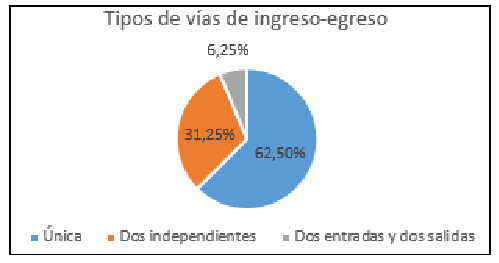
\includegraphics[scale=1]{torta7a.pdf}
	\caption{Proporciones de establecimientos que poseen una sola vía de acceso, dos vías independientes o dos vías de ingreso y dos de egreso.}
	\label{fig:img_torta7a}
\end{figure}


Existen algunos casos particulares, como es el de los establecimientos de menor nivel de afluencia de vehículos que igualmente poseen 2 vías de acceso. Al ser más pequeños, es más complicado maniobrar en el interior y suelen utilizarse ambas vías en forma indistinta. No hay una definida una ruta para la entrada y una para la salida. Igualmente, se los consideró en la categoría de “Dos independientes”. 

\subsection{Disposición del espacio en la zona de ingreso-egreso}

Esta es la característica de los establecimientos en la que mayor diversidad se encuentra. En la mayoría de los casos analizados (11) las vías de ingreso-egreso tienen forma de pasillo, de un largo que permite el acceso de uno o dos vehículos. Sin embargo, mientras que dos de ellos posibilitan la circulación de dos automóviles en paralelo, los nueve restantes se asemejan al garaje de una vivienda y solo permiten la circulación de uno. 

Por otra parte, está el caso de aquellos estacionamientos que no tienen un lugar destinado para la atención de los clientes y la misma se realiza sobre el área de ingreso. Entre los analizados se encuentran dos en esta condición. Además, se tienen establecimientos cuya entrada/salida es en forma de rampa, sobre la cual pueden ubicarse los vehículos para no esperar ser atendidos sobre la calle. En el relevamiento realizado solo hay uno correspondiente a este caso.

Finalmente, están aquellos estacionamientos que poseen más de una vía de entrada-salida, por lo que combinan algunas de las características antes mencionadas. Entre los lugares inspeccionados, se tienen dos con esta particularidad.

\section{Descripción del estacionamiento para ajustes y pruebas   }\label{key:estprotot}
En base a la investigación realizada sobre las características de los establecimientos ubicados en la ciudad de Mar del Plata se decidió simular un estacionamiento en el garaje de una casa que se tenía a disposición. Un croquis del mismo puede observarse en la figura~\ref{fig:img_croquis}.
\begin{figure}[H]
	\centering
	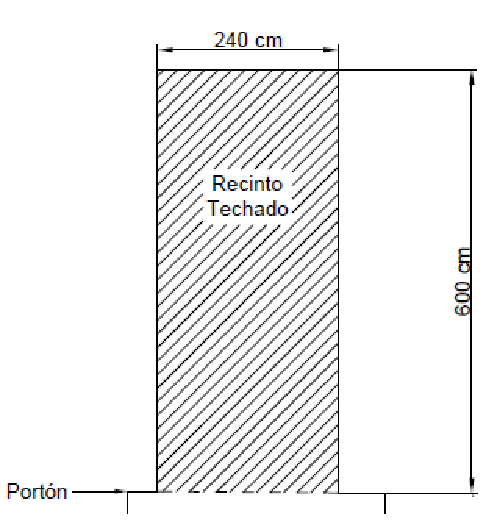
\includegraphics[scale=1]{croquis-est.pdf}
	\caption{Croquis del estacionamiento de prueba.}
	\label{fig:img_croquis}
\end{figure}

La elección realizada se fundamenta en que el establecimiento prototipo posee características similares a la de la mayoría de los que fueron inspeccionados. Las mismas se detallan a continuación:
\begin{itemize}
	\item Tiene forma de pasillo, con espacio para el ingreso de dos vehículos en fila
	\item Es techado y posee luz artificial
	\item El piso está compuesto de baldosas negras lisas. Las mismas, al igual que el piso cemento liso no afectan al momento de tomar las fotografías de la chapa patente
\end{itemize}

\hl{COSAS QUE FALTA HACER LUEGO DE COMPRAR LOS EQUIPOS Y ARMAR EL SISTEMA:}

\hl{-	Ubicacion de las camaras y demas perifericos}

\hl{-	Agregar imagenes?}



